
%(BEGIN_QUESTION)
% Copyright 2010, Tony R. Kuphaldt, released under the Creative Commons Attribution License (v 1.0)
% This means you may do almost anything with this work of mine, so long as you give me proper credit

Suppose we have an Allen-Bradley MicroLogix 1000 controller connected to a pair of momentary-contact pushbutton switches and contactor controlling power to an electric motor as shown in this illustration:

$$\includegraphics[width=15.5cm]{i04662x01.eps}$$

This motor control system has a problem, though: the motor refuses to start when the ``Start'' pushbutton is pressed.  Examine the ``live'' display of the ladder logic program inside this Allen-Bradley PLC to determine what the problem is, assuming an operator is continuously pressing the ``Start'' pushbutton as you examine the program:

$$\includegraphics[width=15.5cm]{i04662x02.eps}$$

Identify at least two causes that could account for all you see here.

\vskip 20pt \vbox{\hrule \hbox{\strut \vrule{} {\bf Suggestions for Socratic discussion} \vrule} \hrule}

\begin{itemize}
\item{} Identify what your next troubleshooting step would be if you were tasked with solving this problem.
\item{} A helpful problem-solving tip is to annotate each contact in the PLC program to show what its real-world function is.  For example, contact {\tt I:0/3} may be labeled ``OL'' because that is the real-world switch status it senses.  Annotate all contacts in this program and explain how this annotation is helpful in analyzing the program.
\item{} Describe the purpose of the contact labeled {\tt O:0/2} in this program, explaining why it is often referred to as a {\it seal-in} contact.
\end{itemize}

\underbar{file i04662}
%(END_QUESTION)





%(BEGIN_ANSWER)

Here are just a couple of possible problems to account for what we are seeing.  There are definitely more possible faults than what are listed here:

\begin{itemize}
\item{} Overload contact tripped (open)
\item{} Wire connecting ``Stop'' switch to OL contact failed open
\end{itemize}

%(END_ANSWER)





%(BEGIN_NOTES)

The missing color in this PLC program is contact {\tt I:0/3}, which is associated with the overload contact.  Since the NO virtual contact is uncolored, its bit state must be 0.  This means the real-world OL contact must be open (tripped), or some other open fault in the circuit causing that input to be de-energized.

\vskip 10pt

Here is a more comprehensive list of possible faults:

\begin{itemize}
\item{} Overload contact tripped (open)
\item{} Wire connecting OL contact to {\tt I:0/3} failed open
\item{} Wire connecting ``Stop'' switch to OL contact failed open
\item{} Input channel {\tt I:0/3} defective on the PLC
\end{itemize}


%INDEX% PLC, relating I/O status to virtual elements (troubleshooting)

%(END_NOTES)


